\documentclass[10pt]{article}
\usepackage[utf8]{inputenc}
\usepackage[T1]{fontenc}
\usepackage{amsmath}
\usepackage{amsfonts}
\usepackage{amssymb}
\usepackage[version=4]{mhchem}
\usepackage{stmaryrd}
\usepackage{graphicx}
\usepackage[export]{adjustbox}
\graphicspath{ {./images/} }

\begin{document}
\section*{CT1 Exercises Architecture}
\begin{enumerate}
  \item Name the main components of the MOCPU and explain their function.
\end{enumerate}

\begin{center}
\begin{tabular}{ll}
Core Registers & \begin{tabular}{l}
$13 \times 32$-bit registers for temporary storage (R0 - R12) \\
$1 \times 32$-bit register for Stack Pointer (SP) (R13) \\
$1 \times 32$-bit register for Link Register (LR) (R14) \\
$1 \times 32$-bit register for Program Counter (PC) (R15) \\
\end{tabular} \\
ALU & \begin{tabular}{l}
Arithmetic Logic Unit \\
Data processing unit for arithmetic and logic operations \\
\end{tabular} \\
Flags & Processor Status Register: Indicates the state of the processor. \\
Control Unit with & \begin{tabular}{l}
Controls execution of an instruction based on the machine \\
code currently stored in the Instruction Register (IR) \\
\end{tabular} \\
Instruction Register &  \\
Bus Interface & \begin{tabular}{l}
Interface between CPU and external System Bus; Bridge \\
between internal and external bus \\
\end{tabular} \\
\end{tabular}
\end{center}

\begin{enumerate}
  \setcounter{enumi}{1}
  \item A processor executes a list of instructions in a predetermined order. Find analogies from everyday life.\\
Baker/cook following a recipe\\
Musician who plays from notes (sheet music)\\
Pilot, who runs through a checklist before takeoff
  \item How many memory bytes can be addressed with an 8-bit memory address? How many with a 16 -bit address? How many with a 32 -bit address?
\end{enumerate}

\begin{verbatim}
8 bit }->256\mathrm{ Bytes
16 bit }->64\mathrm{ KBytes = 65`536 Bytes
32 bit }->4\mathrm{ GBytes = 4'294'967'296 Bytes
\end{verbatim}

\begin{enumerate}
  \setcounter{enumi}{3}
  \item Name 3 instruction types of the MO CPU.
\end{enumerate}

Data transfer\\
Data processing\\
Flow control\\
5. What is the function of the following registers?\\
a. PC

Program counter: Points to the address where the instructions will next be read\\
b. SP

Stack pointer: Points to the memory addresses where the elements are written/read from the stack\\
c. LR

Link Register: Used to keep track of the positions where to jump back (e.g. routines)\\
6. Why is the PC initialized to a defined value at reset? (Although other CPU registers may have an undefined content.)\\
So that fetching of the first instruction can always start at the same (known and predictable) place.\\
7. Name the different parts of a line in assembly code.

Label, mnemonic, operands, comment\\
8. What is a memory map? What is it used for?

It is a graphical layout (map) showing the addresses and sizes of elements that communicate with the CPU (memories, Inputs, Outputs)\\
The memory map helps users to know where each element is (e.g. when writing the appropriate drivers)\\
9. How many byte positions can be addressed by the MO? Which positions in the memory map need to be occupied? Explain your answer.\\
The MO has a 32-Bit address bus. Therefore, it can address 4 GByte $=2^{32}$ Bytes. Positions needed for the initialization of the processor (at Boot) must be covered by the proper elements (memory). Otherwise, there will be no correct start.\\
10. Explain the following terms\\
a. Fetch

Get the instruction from code memory\\
b. Execute

Do what the instructions say\\
c. Word

A 32-bit memory unit (for the MO)\\
d. Half-word

A 16-bit memory unit (for the M0)\\
e. Little endian

A multi-byte representation where the LSByte is at the lower address\\
f. Big endian

A multi-byte representation where the MSByte is at the lower address\\
g. Word Alignment

The address of the multi-byte element is a multiple of the word length ( 4 for the M0)\\
11. A program (code in C) has variables represented as below in the memory map. Determine the decimal values of the variables Var1 .... Var5. Assume Little Endian representation.

\begin{center}
\begin{tabular}{|c|c|c|}
\hline
Address & Byte content (decimal, hex, binary) & Variable \\
\hline
0x2FFF'FFF7 & 0x45 &  \\
\hline
0x2FFF'FFF8 & 0xE2 & Var4 (16-bit short) \\
\hline
0x2FFF'FFF9 & 01100010 (binary) &  \\
\hline
0x2FFF'FFFA & 213 &  \\
\hline
0x2FFF'FFFB & 25 &  \\
\hline
0x2FFF'FFFC & 0x65 & Var3 (32-bit unsigned integer) \\
\hline
0x2FFF'FFFD & 10101101(binary) &  \\
\hline
0x2FFF'FFFE & 0xA3 &  \\
\hline
0x2FFF'FFFF & 0x82 &  \\
\hline
0x3000'0000 & 0xA2 & Var5 (32-bit integer) \\
\hline
0x3000'0001 & 34 &  \\
\hline
0x3000'0002 & 0x54 &  \\
\hline
0x3000'0003 & 0xFF &  \\
\hline
0x3000'0004 & 0x92 & Var2 (unsigned char) \\
\hline
$0 \times 3000{ }^{\prime} 0005$ & 0x03 & Var1 (char) \\
\hline
\end{tabular}
\end{center}

Var1 =\\
Var1 $=0 \times 03=3 d$ (it is 8-bit unsigned)

Var2 =\\
Var2 $=0 \times 92=146 \mathrm{~d}$ (it is 8 -bit unsigned)

Var3 =\\
Var3 $=0 \times 82 A 3 A D 65=+2^{\prime} 191^{\prime} 764$ '837d (it is 32-bit unsigned!!)

Var4 =\\
Var4 $=0 \times 62 \mathrm{E} 2=+25$ '314d (it is 16 -bit signed)

Var5 =\\
Var5 $=0 x F F 5422 A 2=-1^{\prime} 1263$ '326 (it is 32-bit signed)\\
(-2'147'483'648 + 2'136'220'322)

How would the same variable values be stored on a Big Endian platform? Fill in the table.

\begin{center}
\begin{tabular}{|c|c|c|}
\hline
Address & Byte content (decimal, hex, binary) & Variable \\
\hline
0x2FFF'FFF7 & 0x45 &  \\
\hline
0x2FFF'FFF8 & 01100010 (binary) & Var4 (short) \\
\hline
0x2FFF'FFF9 & 0xE2 &  \\
\hline
0x2FFF'FFFA & 213 (or 25) &  \\
\hline
0x2FFF'FFFB & 25 (or 213) &  \\
\hline
0x2FFF'FFFC & 0x82 & Var3 (32-bit unsigned integer) \\
\hline
0x2FFF'FFFD & 0xA3 &  \\
\hline
0x2FFF'FFFE & 10101101(binary) &  \\
\hline
0x2FFF'FFFF & $0 \times 65$ &  \\
\hline
0x3000'0000 & 0xFF & Var5 (32-bit integer) \\
\hline
0x3000'0001 & 0x54 &  \\
\hline
0x3000'0002 & 34 &  \\
\hline
0x3000'0003 & 0xA2 &  \\
\hline
0x3000'0004 & $0 \times 92$ & Var2 (unsigned char) \\
\hline
0x3000'0005 & $0 \times 03$ & Var1 (char) \\
\hline
\end{tabular}
\end{center}

We are not told if 25 / 213 form a unit or not. Therefore, it can be both ways.\\
12. Which 3 memory areas (sections) can be differentiated for a program? What will be stored in the individual areas? In which memory type can the areas be located?\\
CODE read-only $\rightarrow$ RAM or ROM\\
Machine instructions, constants\\
DATA read-write $\rightarrow$ RAM\\
Global variables, static variables and heap in C\\
STACK read-write $\rightarrow$ RAM\\
Procedure calls / passing of parameters, local variables\\
13. Assume that the following memory areas are used when executing a program:

\begin{itemize}
  \item Code: $0 \times 20000000$ to $0 x 200001 F F$
  \item Data: 0x20000200 to 0x200002FF
  \item Stack: 0x20000300 to 0x200003FF
\end{itemize}

Draw an appropriate memory map and draw the three sections. Label the first and last addresses for each area. How many storage locations does each of the areas contain?\\
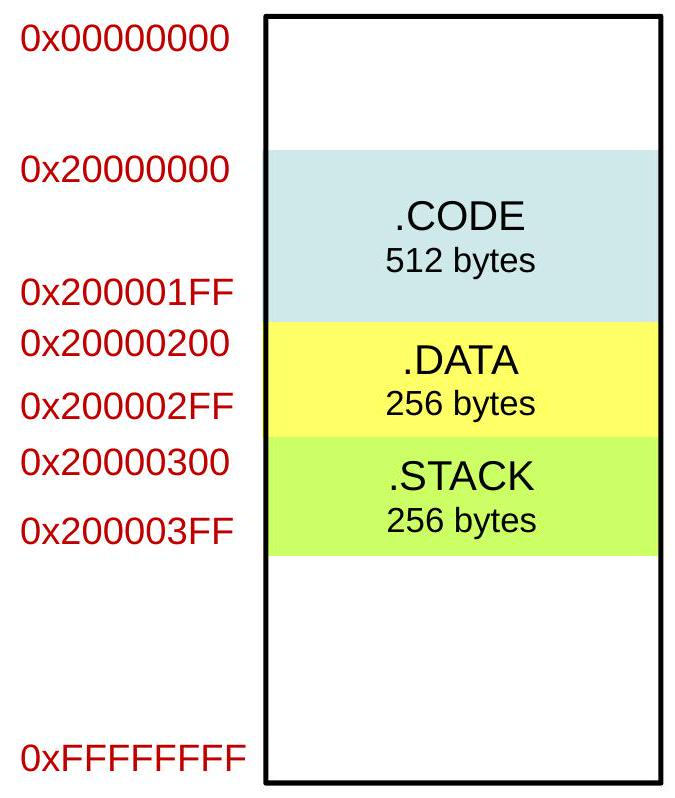
\includegraphics[max width=\textwidth, center]{2025_01_02_5d04f07cd96c1366bf1bg-5}


\end{document}